%!TEX root = lec07_documents.tex

\begin{frame}{The Web As Of Not Too Long Ago}

HTML: HyperText Markup Language
\begin{itemize}[-,noitemsep,topsep=-5pt]
\item \alert{W3C Standard} implemented by most browsers
\item Still not fully supported across all platforms
\end{itemize}

\vskip1em

HTML enabled mass publishing of human-generated content (e.g., news, blogs, etc.) and server-generated content (by pulling data out of a relational database)
\begin{itemize}[-,topsep=-5pt]
\item PHP, JavaScript, ASP...
\end{itemize}

\vskip1em

HTML was designed to present content for  \textbf{human consumption}. That is, it specifies how to make content look nice on the browser, not what that content \textbf{means}.

\end{frame}

\lstset{
	style=markup,
    emph=[1]{%
        name,content
    },
    emphstyle=[1]{\color{sqlColor}}
}

\newsavebox\movieHMLexample
\begin{lrbox}{\movieHMLexample}
\begin{lstlisting}[style=markup]
<HTML>
 <head>
  <title>Movie List</title>
  <meta name="author" 
        content="John Smith">
 </head>
 <body>
  <h1> Movie List </h1>
  <p> <i> Ghostbusters </i> (1984)
     <br> <b> Ivan Reitman </b>
     <br> With Bill Murray, 
           Sigourney Weaver

  <p> <i> Groundhog Day </i> (1993)
     <br> <b> Harold Ramis </b>
     <br> With Bill Murray, 
           Andie MacDowell
 </body>
</HTML>
\end{lstlisting}
\end{lrbox}


\begin{frame}[fragile]{Markup Languages}

\vskip1em

\begin{columns}[onlytextwidth]
\begin{column}{0.55\textwidth}
Markup: annotations (tags) in a plain text document

\vskip1em
HTML's markup vocabulary is \textbf{fixed} and tags have \alert{pre-specified semantics}:
\begin{itemize}[-,noitemsep,topsep=-5pt]
\item \lstinline[style=markup]!<head>! tag is for metadata while the ``data'' goes into the \lstinline[style=markup]!<body>! tag.
\item HTML has tags for choosing fonts and colors, drawing tables, adding line breaks, paragraphs, hierarchical headers, etc.
\end{itemize}

\vskip1em
Tags need not be closed in HTML
\end{column}
\begin{column}{0.4\textwidth}
\begin{tikzpicture}
\node {\scalebox{0.85}{\usebox\movieHMLexample}};

\onslide<2-|handouts:1>{
  \node (markup) at (0,4) [color=blue] {markup};
  \node (c1) at (-1.75,3.5) [color=blue,circle] {};
  \node (c2) at (1,3) [color=blue,circle] {};
  \draw [blue,thick,->,>=stealth] (markup) -- (c1); \draw [blue,thick,->,>=stealth] (markup) -- (c2);
}
\onslide<3|handouts:1>{
  \node (content) at (1,1.5) [color=red] {content};
  \node (c3) at (-0.5,0.75) [color=blue,circle] {};
  \draw [red,thick,->,>=stealth] (content) -- (c3);
}
\end{tikzpicture}
\end{column}
\end{columns}

\end{frame}


\newsavebox\movieXMLexample
\begin{lrbox}{\movieXMLexample}
\begin{lstlisting}[style=markup]
<movies>
 <meta name="author" 
        content="John Smith"/>
 <movie>
  <title>Ghostbusters</title>
  <year>1984</year>
  <director>Ivan Reitman</director>
  <cast>
   <actor>Bill Murray</actor>
   <actor>Sigourney Weaver</actor>
  </cast>
 </movie>
 <movie>
  <title>Groundhog Day</title>
  <year>1993</year>
  <director>Harold Ramis</director>
  <cast>
     <actor>Bill Murray</actor>
     <actor>Andie MacDwowell</actor>
  </cast>
 </movie>
</movies>
\end{lstlisting}
\end{lrbox}

\begin{frame}[fragile]{The Extensible Markup Language}

\vskip2em
\begin{columns}[onlytextwidth]
\begin{column}{0.54\textwidth}
W3C~recommendation markup language that allows user-defined vocabulary.
\begin{itemize}[-,topsep=-5pt]
\item Programmers choose their own tags.
\item Applications can interpret the tags any way they want.
\end{itemize}

\vskip2em

XML tags must always be closed in the reverse order in which they are opened.
\begin{itemize}[-,topsep=-5pt]
\item Ensures the document can be parsed correctly.
\end{itemize}
\end{column}
\begin{column}{0.4\textwidth}
\scalebox{0.75}{\usebox\movieXMLexample}
\end{column}
\end{columns}
\end{frame}

\begin{frame}{XML vs HTML}

In summary:

\begin{itemize}[-]
\item Both are markup languages that apply to plain text documents
\item HTML has a finite and pre-defined set of tags; with XML, you can choose your own set of tags
\item HTML and XML documents can be represented as trees (through the Document Object Model)
\item Closing tags in HTML is optional; the browser makes educated guesses about the shape of the tree
\item Closing tags in XML is required; there is only one DOM tree that represents a well-formed XML document
\end{itemize}
\end{frame}


\begin{frame}{XML Standards}

XSL/XSLT: presentation and transformation
\begin{itemize}[-,topsep=-05pt,noitemsep]
\item ex: transforming XML into plain HTML content
\end{itemize}

RDF: resource description framework 
\begin{itemize}[-,topsep=-5pt,noitemsep]
\item used for describing meta-data about XML documents
\item foundation for the Semantic Web
\end{itemize}

Xpointer/Xlink: specifies links across documents and elements

DOM: Document Object Model for representing XML documents
\begin{itemize}[-,topsep=-5pt,noitemsep]
\item implementations in all popular languages
\end{itemize}


SAX: Simple API for XML parsing
\begin{itemize}[-,topsep=-5pt,noitemsep]
\item event-based framework
\item implementations in all popular languages
\end{itemize}
\end{frame}

\begin{frame}{What is XML good for?}

\begin{wrapfigure}[6]{r}{0.4\textwidth}
\vspace*{-3em}
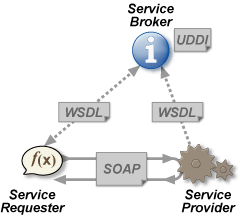
\includegraphics[width=0.4\textwidth]{figures/Webservices.png}
\end{wrapfigure}

\textbf{Web Services}\footnote{\url{https://en.wikipedia.org/wiki/Web_service}} are software systems designed to support interoperable machine-to-machine interaction over the Web (or some other network). 

With Service-Oriented Architectures, an entire application can be implemented by calling services that perform specific tasks.

XML is used to encode messages between the application (the requester) and the service provider. The application can choose among many providers offering the same service.

See CMPUT401!
\end{frame}


\begin{frame}{What is XML good for?}

\vskip1em

\begin{columns}[onlytextwidth]
\begin{column}{0.38\textwidth}
\textbf{Ajax}\footnotemark, short for asynchronous JavaScript and XML, is a set of web development techniques using many web technologies on the client side to create asynchronous web applications.

\vskip1em

See CMPUT404!
\end{column}
\begin{column}{0.6\textwidth}
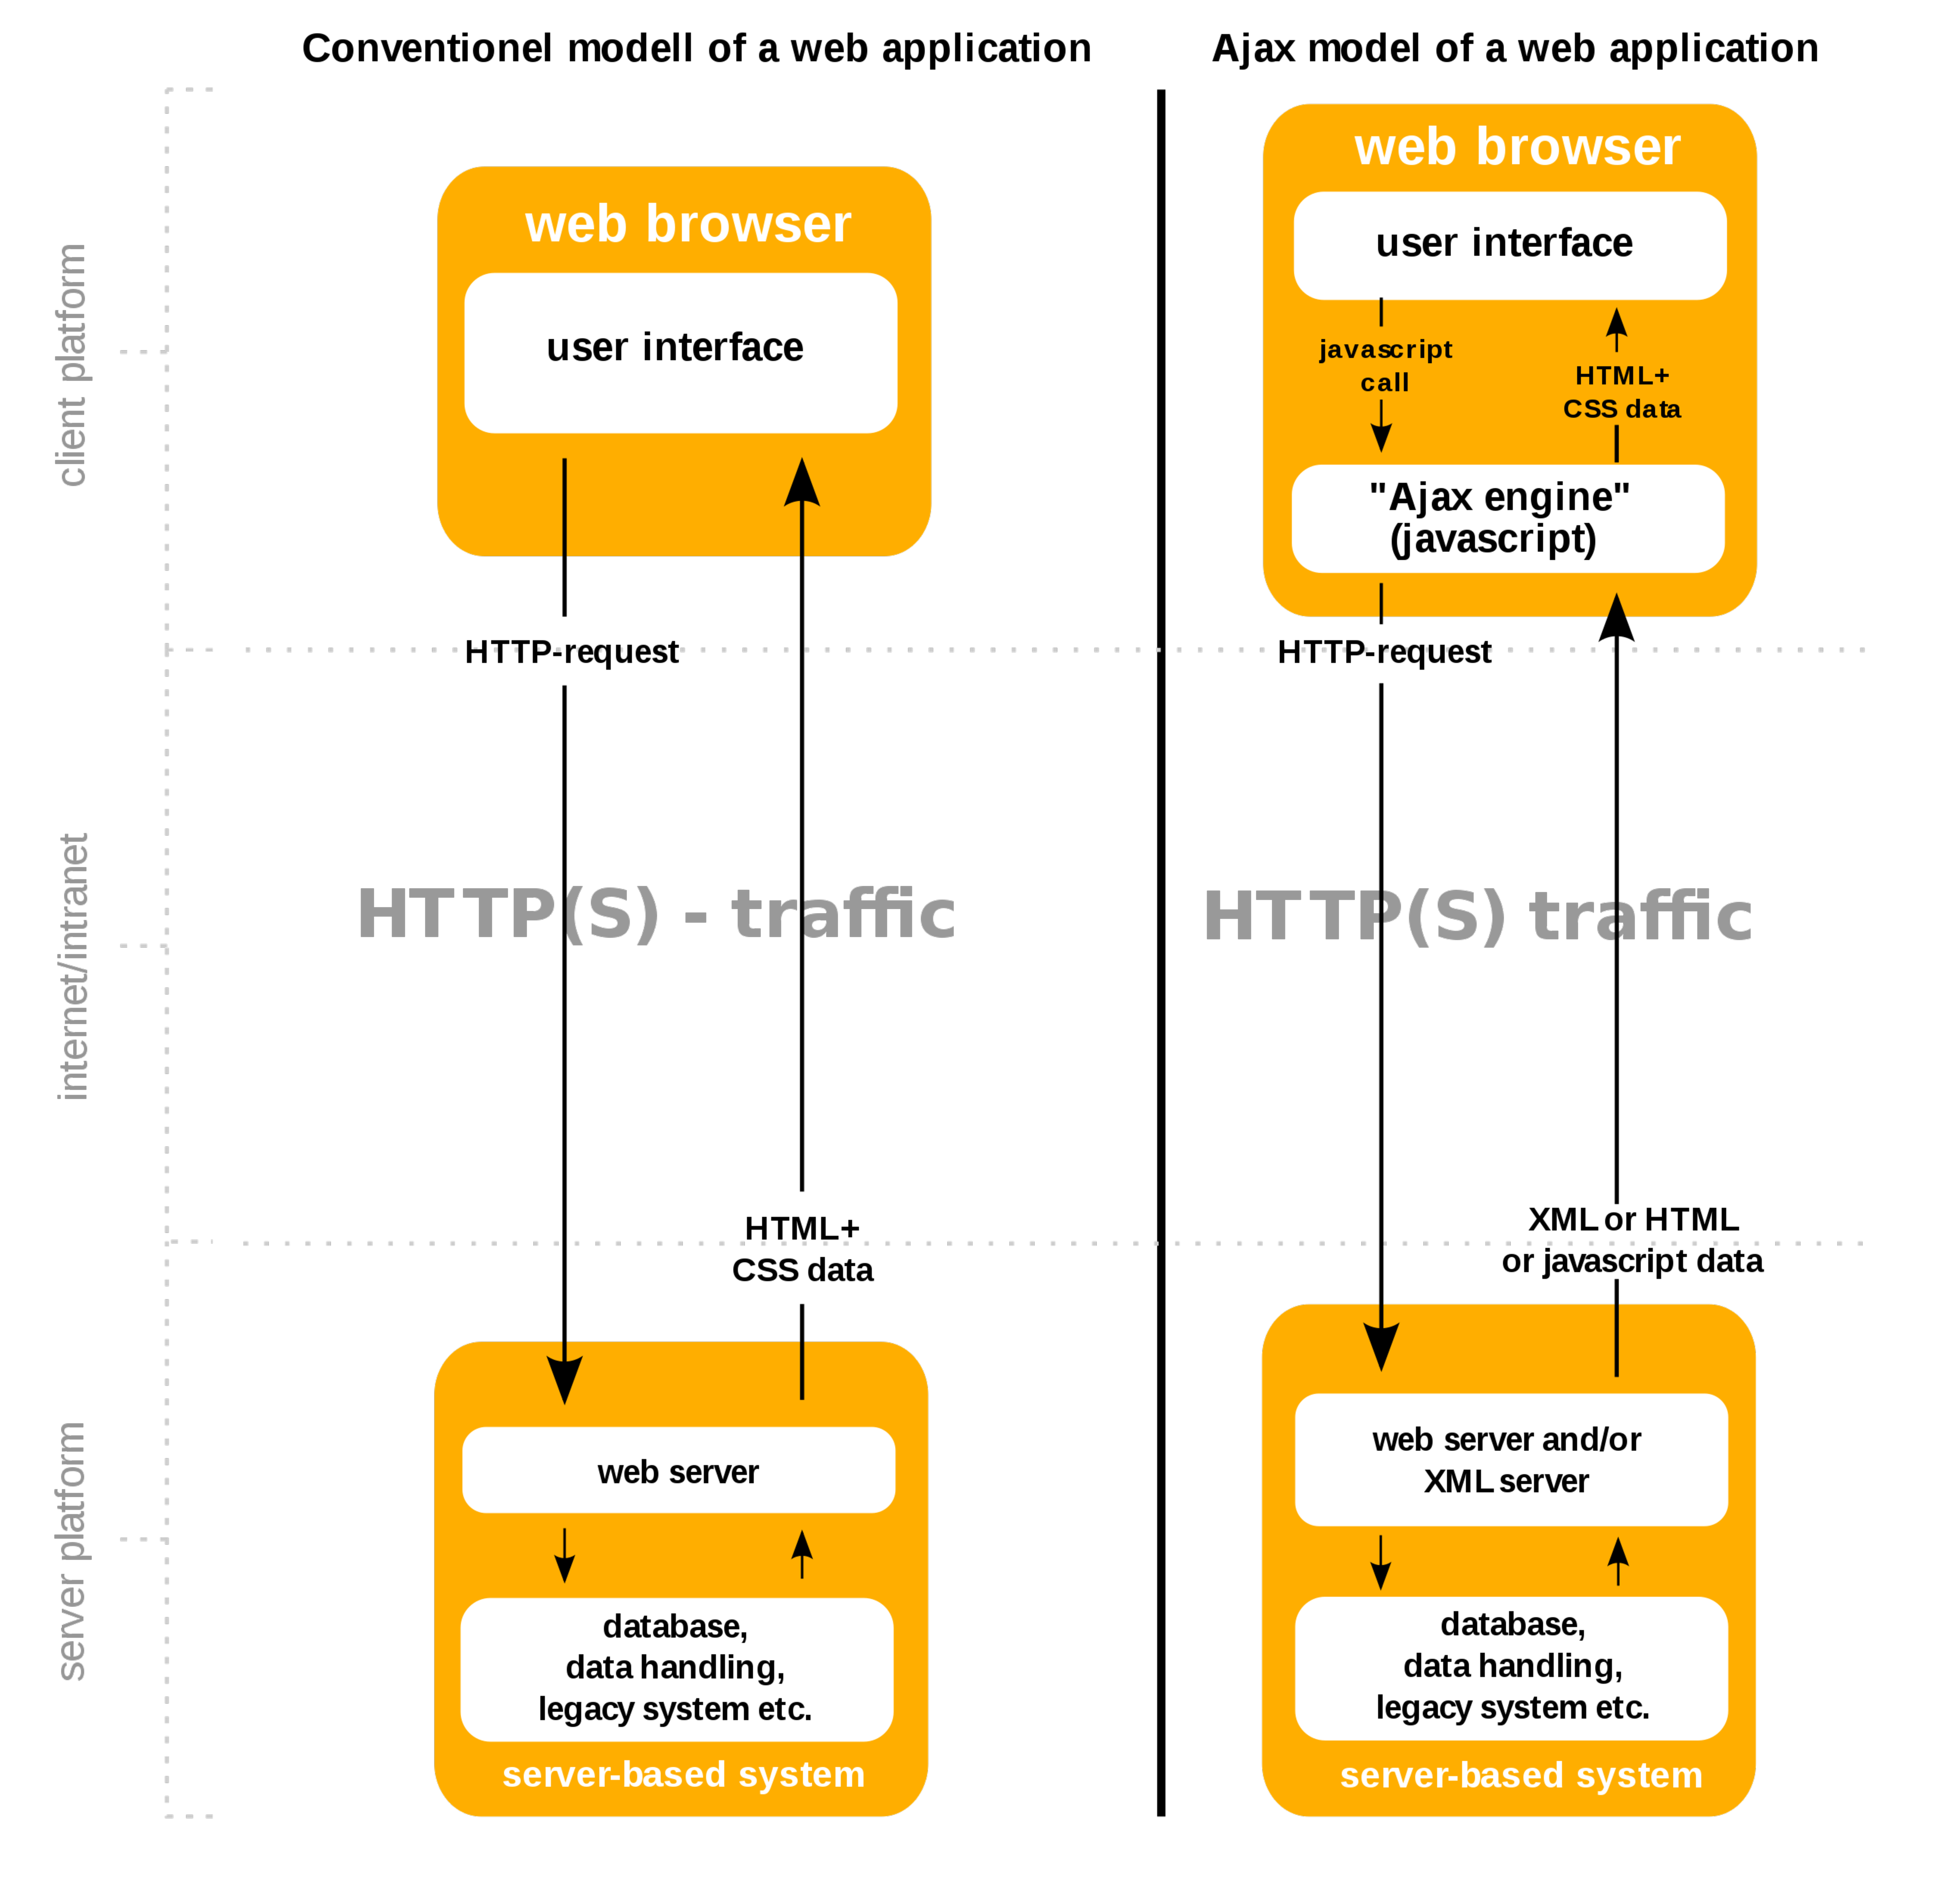
\includegraphics[width=1.2\textwidth]{figures/2560px-Ajax-vergleich-en.pdf}
\end{column}
\end{columns}

\footnotetext{\url{https://en.wikipedia.org/wiki/Ajax_(programming)}}
\end{frame}

\begin{frame}{What is XML good for?}

XML is great for \alert{encoding and exchanging data} \textbf{between} existing (database-backed) \textbf{systems}.

Why?
\begin{itemize}[-]
\item XML is \textbf{text-based}: it is a lot easier to read or write text files than binary files (e.g., the programmer can inspect the file while debugging).
\item It enables incremental data sharing formats; once two systems can talk, it is easy to extend the markup to support more systems.
\item XML is an open standard, supported by many tools (and developers).
\end{itemize}

\end{frame}

\newsavebox\exampleXMLDTD
\begin{lrbox}{\exampleXMLDTD}
\begin{lstlisting}[style=markup]
<?xml version="1.0" encoding="UTF-8"?>
<?xml-stylesheet type="text/css" href="movies.css"?>
<!DOCTYPE movies SYSTEM "http://movies.org/movies.dtd">
<movies>
 <movie> 
  <title>Ghostbusters</title> <year>1984</year>
  <director>Ivan Reitman</director>
  <cast>
    <actor>Bill Murray</actor>
<!-- this is a comment -->
    <actor>Sigourney Weaver</actor>
  </cast>
 </movie>
</movies>
\end{lstlisting}
\end{lrbox}


\begin{frame}[fragile]{What Does XML Look Like?}

\vspace*{-2em}
\begin{center}
\begin{tikzpicture}
\node (fig) at (0,0) [anchor=north west] {\scalebox{0.75}{\usebox\exampleXMLDTD}};
\node (c1) at (0.25,-0.25) [circle,blue] {};
\node (c2) at (0.25,-1) [circle,blue] {};
\node (c3) at (6,-0.6) [circle,blue] {};
\node (c4) at (0.25,-3.5) [circle,blue] {};
\node (enc) at (-2,0) [rectangle,draw,blue,align=center,text width=1.75cm] {\footnotesize encoding};
\draw[blue,thick,->,>=stealth] (enc) -- (c1);
\node (dtd) at (-2,-1) [rectangle,draw,blue,align=center,text width=1.75cm] {\footnotesize document\\[-0.75em] type};
\draw[blue,thick,->,>=stealth] (dtd) -- (c2);
\node (css) at (7,0.25) [rectangle,draw,blue,align=center,text width=1.75cm] {\footnotesize Stylesheet};
\draw[blue,thick,->,>=stealth] (css) -- (c3);
\node (com) at (-2,-3) [rectangle,draw,blue,align=center,text width=1.75cm] {\footnotesize comment};
\draw[blue,thick,->,>=stealth] (com) -- (c4);
\end{tikzpicture}
\end{center}

An XML element consists of an opening tag, the corresponding closing tag, and everything that goes in between them

The \alert{content of the element} is what goes between the tags\\
~$-$~~may consist of: text, other elements, or a mix of both

\end{frame}

\begin{frame}[fragile]{Representing relational data as XML}

XML is a quite popular format for exchanging relational data, because most applications use RDBMSs. In fact, there is even a standard called SQL/XML that helps with that. (More on this later).

\vskip1em

\begin{columns}[onlytextwidth]
\begin{column}{0.45\textwidth}
An obvious solution would be to map each row of each relation to an element:

\vskip1em

\scalebox{0.75}{\usebox\MovieTable}
\end{column}
\begin{column}{0.45\textwidth}
\begin{lstlisting}[style=markup,basicstyle=\ttfamily\scriptsize]
...
<Movie>
 <row> <title>Ghostbusters</title>
    <year>1984</year>
    <imdb>7.8</imdb>
    <director>Ivan Reitman</director>
 </row>
  <row> <title>Big</title>
  ... 
  </row>
 ...
</Movie>
...
\end{lstlisting}
\end{column}
\end{columns}
\end{frame}

\begin{frame}[fragile]
XML does not suffer from the 1NF limitation: elements can be multi-valued. Thus we can ``nest'' a table inside another (e.g., if there is a PK/FK relationship between them):

\begin{center}
\begin{lstlisting}[style=markup][basicstyle=\ttfamily\scriptsize]
...
<Movie>
 <row> <title>Ghostbusters</title>
    <year>1984</year>
    <imdb>7.8</imdb>
    <director>Ivan Reitman</director>
    <cast>
      <actor>Bill Murray</actor> <role>Dr. Venkman</role>
      <actor>Sigourney Weaver</actor> <role>Dana Barret</role>
    </cast>
 </row>
 ...
</Movie>
...
\end{lstlisting}
\end{center}

\end{frame}

\begin{frame}[fragile]{Attributes, data and meta-data}

\begin{center}
\footnotesize
\begin{lstlisting}[style=markup]
<bibliography> 
   <book -|isbn|-="046509760X">
        <title>The Book of Why</title>
        <author>Pearl</author>
        <author>Mackenzie</author>
        <publisher>Basic Books</publisher>
        <price -|currency|-="CDN">45.00</price>
   </book>
</bibliography>
\end{lstlisting}
\end{center}

Attributes may be added to describe, identify or \alert{link} elements
\begin{itemize}[-,noitemsep]
\item \lstinline{-|isbn|-} identifies the book
\item \lstinline{-|currency|-} explains that the price is in Canadian dollars
\end{itemize}

In principle, attributes should be \emph{metadata}; but it is hard to distinguish data from metadata sometimes.
\end{frame}



\newsavebox\PandPXML
\begin{lrbox}{\PandPXML}
\begin{lstlisting}[style=markup][linewidth=0.7\textwidth,breaklines=true]
<book>
 <title>Pride And Prejudice</title>
 <chapter>
  <title>Chapter 1</title>
  <p>It is a truth universally acknowledged, 
  that a single man in possession of a good 
  fortune must be in want of a wife. </p>
  <p>...</p>
  ...
 </chapter>
 <chapter>
  <title>Chapter 2</title>
  <p>Mr. Bennet was among the earliest of 
  those who waited on Mr. Bingley...</p>
  <p>...</p>
  ...
 </chapter>
 ...
</book>
\end{lstlisting}
\end{lrbox}

\begin{frame}[fragile]{Document Order}

\vskip2em

\begin{columns}[onlytextwidth]
\begin{column}{0.5\textwidth}
XML is meant to encode \alert{documents}, thus, unlike with tuples in a table, the ordering of the elements in a document is important.
\begin{itemize}[-,topsep=-0.5pt,noitemsep]
\item Think about reading your favorite book in a random order of chapters!
\item XML Storage systems must preserve element ordering.
\end{itemize}

\vskip1em

As we will see later, we can ask queries involving element order.

\end{column}
\begin{column}{0.45\textwidth}
\scalebox{0.75}{\usebox\PandPXML}
\end{column}
\end{columns}
\end{frame}

\begin{frame}[fragile]{XML Elements are Trees}

The nesting of elements naturally induce a tree, often called the Document Object Model (DOM) tree:

\begin{lstlisting}[style=markup][basicstyle=\ttfamily\scriptsize]
   <book>
        <title>The Book of Why</title>
        <author>Pearl</author>
        <author>Mackenzie</author>
        <publisher>Basic Books</publisher>
   </book>
\end{lstlisting}

\small
\begin{tikzpicture}[every node/.style={font=\footnotesize\ttfamily}]
\node (book) at (0,0) {\textcolor{accent}{<book>}};
\node (title) [below left=15pt and 65pt of book] {\textcolor{accent}{<title>}};
\node (a1) [right= 50pt of title] {\textcolor{accent}{<author>}};
\node (a2) [right= 30pt of a1] {\textcolor{accent}{<author>}};
\node (publisher) [right= 30pt of a2] {\textcolor{accent}{<publisher>}};
\node (t) [below= 10pt of title] {The Book of Why};
\node (at1) [below= 10pt of a1,text width=35pt] {Pearl};
\node (at2) [below= 10pt of a2,text width=35pt] {Mackenzie};
\node (p) [below= 10pt of publisher] {Basic Books};
\draw[->] (book) -- (title); \draw[->] (book) -- (a1); \draw[->] (book) -- (a2); \draw[->] (book) -- (publisher);
\draw[->] (title) -- (t);
\draw[->] (a1) -- (at1); \draw[->] (a2) -- (at2); \draw[->] (publisher) -- (p);
\end{tikzpicture}

Edges in the tree represent the \textbf{parent-child} relationship, from which we can derive other relationships: ancestor, descendant and sibling.

\end{frame}



\begin{frame}[fragile]{Constraints? Schemas?}

\begin{BOX}{Document Type Definitions (DTDs)}
Originated from SGML\footnotemark; uses \alert{regular expressions} to specify which elements can be nested within others and simple rules to specify attributes.
\end{BOX}

\footnotetext{Standard Generalized Markup Language--\url{https://en.wikipedia.org/wiki/Standard_Generalized_Markup_Language}}


\begin{BOX}{XML Schema}
Borrow best practices from databases and programming languages; adds support for specifying data types for the various elements.

\vskip0.5em

Strictly more powerful than DTDS: you can always rewrite a DTD as a schema, but not the other way around.
\end{BOX}
\end{frame}


\lstset{language=DTD}

\newsavebox\DTDexample
\begin{lrbox}{\DTDexample}
\begin{lstlisting}
<!DOCTYPE bibliography [
 <!ELEMENT bibliography (book-|*|-)>
 <!ELEMENT book (title, author-|+|-, publisher, price-|?|-)>
 <!ATTLIST book isbn -:ID #REQUIRED:->
 <!ELEMENT title (-:#PCDATA:-)>
 <!ELEMENT author (-:#PCDATA:-)>
 <!ELEMENT publisher (-:#PCDATA:-)>
 <!ELEMENT price (-:#PCDATA:-)
 <!ATTLIST price currency -:CDATA #IMPLIED:-> 
]>
\end{lstlisting}
\end{lrbox}


\begin{frame}[fragile]{DTDs}

\vskip1em

\begin{columns}[onlytextwidth]
\begin{column}{0.35\textwidth}
\lstinline{ELEMENT} rules specify what can go in an element via \alert{regular expressions}.

\vspace*{2em}
\end{column}
\begin{column}{0.6\textwidth}
\scalebox{0.8}{\usebox\DTDexample}
\end{column}
\end{columns}


Each \lstinline{bibliography} element can contain zero or more \lstinline{book} elements and nothing else.

A \lstinline{book} element \textbf{must} have a \lstinline{title}, at least one \lstinline{author}, and a \lstinline{publisher}; it may also have a \lstinline{price} element.

Elements \lstinline{title}, \lstinline{author}, \lstinline{publisher}, and \lstinline{price} can contain only ``parsed character data'' (\lstinline[language=DTD]!-:#PCDATA:-!), which is XML for ``text''.

\end{frame}

\begin{frame}[fragile]{Validation of \lstinline{ELEMENT} Rules}

\textbf{Defn}: an element is valid if its \emph{content} matches the regular expression associated with its name in the DTD.

\textbf{Defn}: a document is valid if all of its elements are valid.


For validation purposes, the \emph{content} of element $x$ is one of\footnote{XML allows elements to have \emph{mixed} content as well: that is, elements interspersed with text. We will ignore such content in CMPUT391 for simplicity.}:\\
 - a string formed by the labels of the children of $x$\\
 - \lstinline[language=DTD]{-:#PCDATA:-} if the element contains only text

\begin{block}{Example: \lstinline[style=markup]{<cast><actor>Bill Murray</actor></cast>}}
The content of the \lstinline[style=markup]{<cast>} element is \lstinline[style=markup]{actor}, and the content of \lstinline[style=markup]{<actor>} is \lstinline[language=DTD]{-:#PCDATA:-}.
\end{block}
\end{frame}

\begin{frame}[fragile]

\vskip2em

\begin{lstlisting}[style=markup][basicstyle=\ttfamily\scriptsize]
<bibliography>
    <book>
        <title>The Book of Why</title>
        <author>Pearl</author>
        <author>Mackenzie</author>
        <publisher>Basic Books</publisher>
    </book>
</bibliography>
\end{lstlisting}

% \small
% \begin{tikzpicture}[every node/.style={font=\footnotesize\ttfamily}]
% \node (book) at (0,0) {\textcolor{accent}{<book>}};
% \node (title) [below left=15pt and 65pt of book] {\textcolor{accent}{<title>}};
% \node (a1) [right= 50pt of title] {\textcolor{accent}{<author>}};
% \node (a2) [right= 30pt of a1] {\textcolor{accent}{<author>}};
% \node (publisher) [right= 30pt of a2] {\textcolor{accent}{<publisher>}};
% \node (t) [below= 10pt of title] {The Book of Why};
% \node (at1) [below= 10pt of a1,text width=35pt] {Pearl};
% \node (at2) [below= 10pt of a2,text width=35pt] {Mackenzie};
% \node (p) [below= 10pt of publisher] {Basic Books};
% \draw[->] (book) -- (title); \draw[->] (book) -- (a1); \draw[->] (book) -- (a2); \draw[->] (book) -- (publisher);
% \draw[->] (title) -- (t);
% \draw[->] (a1) -- (at1); \draw[->] (a2) -- (at2); \draw[->] (publisher) -- (p);
% \end{tikzpicture}

\vskip2em

Is the element above valid?

\begin{lstlisting}[basicstyle=\ttfamily\scriptsize]
 <!ELEMENT bibliography (book-|*|-)>
 <!ELEMENT book (title, author-|+|-, publisher, price-|?|-)>
 <!ELEMENT title (-:#PCDATA:-)>
 <!ELEMENT author (-:#PCDATA:-)>
 <!ELEMENT publisher (-:#PCDATA:-)>
 <!ELEMENT price (-:#PCDATA:-)
\end{lstlisting}

\end{frame}

\begin{frame}[fragile]

\vskip1em

\begin{columns}[onlytextwidth]
\begin{column}{0.35\textwidth}
\lstinline{ATTLIST} rules specify whether attributes are required, and whether they can be used as identifiers.

\vspace*{2em}
\end{column}
\begin{column}{0.6\textwidth}
\scalebox{0.8}{\usebox\DTDexample}
\end{column}
\end{columns}


\lstinline[language=DTD]!-:CDATA:-! means ``character data''. Attributes cannot have elements or other attributes as their value.

\lstinline[language=DTD]!-:#REQUIRED:-! indicates the attribute must be present; while \lstinline[language=DTD]!-:#IMPLIED:-! means the attribute is optional.

Finally, \lstinline[language=DTD]!-:#ID:-! indicates that the value of the attribute must be unique \textbf{within the document}.

\end{frame}


\newsavebox\bibliographyDTD
\begin{lrbox}{\bibliographyDTD}
\begin{lstlisting}[language=DTD,basicstyle=\ttfamily\scriptsize]
<!DOCTYPE bibliography [
 <!ELEMENT bibliography (book-|*|-)>
 <!ELEMENT book (title, author-|+|-, publisher, price-|?|-)>
 <!ATTLIST book isbn ID #REQUIRED
                -|sequel IDREF|- #IMPLIED>
 <!ELEMENT title (#PCDATA)>
 <!ELEMENT author (#PCDATA)>
 <!ELEMENT publisher (#PCDATA)>
 <!ATTLIST -|publisher website|- ID #IMPLIED>
 <!ELEMENT price (#PCDATA)
 <!ATTLIST price currency CDATA #IMPLIED> 
]>
\end{lstlisting}
\end{lrbox}

\begin{frame}[fragile]{\lstinline[language=DTD]!-:ID:-! and \lstinline[language=DTD]!-:IDREF:-! attributes}

\lstinline[language=DTD]!-:#ID:-! and \lstinline[language=DTD]!-:#IDREF:-! attributes are ``like'' keys and foreign keys, but not quite, because their scope is the entire document (instead of individual tables).

\vskip1em

\usebox\bibliographyDTD

% \lstset{language=DTD}

The (optional) \lstinline[language=DTD]!-|sequel|-! must match the value of some \lstinline[language=DTD]!-:#ID:-! attribute.
\end{frame}


\newsavebox\validATTexample
\begin{lrbox}{\validATTexample}
\begin{lstlisting}[style=markup]
<bibliography>
 <book isbn="1234"> 
  ...
  <publisher website="abc.ca">
   ...
  </publisher>
 </book>
 <book isbn="5678" sequel="1234">
  ...
  <publisher>...</publisher>
 </book>
 <book isbn="xyz" sequel="abc.ca">
  ...
 </book>
<bibliogaphy>
\end{lstlisting}
\end{lrbox}

\newsavebox\dtdATTexample
\begin{lrbox}{\dtdATTexample}
\begin{lstlisting}[language=DTD]
<!DOCTYPE bibliography [
 ...
 <!ATTLIST book isbn -:ID #REQUIRED:-
                -|sequel IDREF #IMPLIED|->
 <!ATTLIST -|publisher website ID #IMPLIED|->
 <!ATTLIST price currency -:CDATA #IMPLIED:-> 
]>
\end{lstlisting}
\end{lrbox}


\begin{frame}[fragile]{Validation of \lstinline[language=DTD]!ATTLIST! Rules}

A \lstinline[language=DTD]!-:#REQUIRED:-! attribute must be present, otherwise the element (and the document) is invalid. An \lstinline[language=DTD]!-:#IMPLIED:-! attribute is optional.

The value of an \lstinline[language=DTD]!-:#ID:-! attribute be unique within the document, while the value of an \lstinline[language=DTD]!-:#IDREF:-! attribute must match some \lstinline[language=DTD]!-:#ID:-! attribute.

\vskip1em

\begin{columns}[onlytextwidth]
\begin{column}{0.5\textwidth}
\scalebox{0.75}{\usebox\dtdATTexample}

\vskip1em

Note that, counter to what you would expect, we cannot specify that \lstinline!-|sequel|-! must match the \lstinline!-|isbn|-! of another book!
\end{column}
\begin{column}{0.4\textwidth}
\scalebox{0.75}{\usebox\validATTexample}
\end{column}
\end{columns}

\end{frame}


\begin{frame}{DTDs}

DTDs are enough for describing documents, but have many shortcomings if used to describe relational data.

\begin{itemize}[-]
\item Can ``simulate'' unary keys (ID attributes), but there is no support for n-ary keys.

\item No support for inclusion dependencies; IDREF attributes are not restricted to specific ID attributes.

\item Only data type is ``text''.

\item Element name and ``type'' (regular expression on child labels) are associated globally (i.e., independently of context).

\end{itemize}
\end{frame}

\begin{frame}[fragile]{XML Schema}
\begin{itemize}[-]
\item In XML format.
\item Element types are contextualized.\\
 - Ex: different book elements may have different types depending on the label of their parent.
\item Defines several primitive data types (integers, strings, dates, etc.) and allows user-defined data types.
\item Supports all common data types and the specification of domains (like SQL CHECK constraints)
\item Supports proper keys (including n-ary) and foreign keys.
\item Inheritance (extension or restriction).
\item Element-type reference constraints.
\end{itemize}
\end{frame}

\begin{frame}[fragile]{(Simplified) Example XML Schema}

\begin{lstlisting}[style=markup,basicstyle=\ttfamily\scriptsize]
<schema version="1.0" xmlns="http://www.w3.org/1999/XMLSchema">
 <element name="book">
   <complexType>
     <attribute name="isbn" type="string" use="required"/>
     <element name="title" type="string"/>
 
     <element name="author" minOccurs="1" maxOccurs="7" type="author_type"/>

      <element name="publisher" type="string" />

      <element ref="price" minOccurs="0" maxOccurs="1">
       <complexType>
          <simpleContent>
            <extension base="float"/>
            <attribute name="currency" type="string" use="optional"/>
          </simpleContent>
       </complexType>
      </element>
     </complexType>
 </element>
</schema>
\end{lstlisting}

\end{frame}